% !TeX root = ../main.tex
% Add the above to each chapter to make compiling the PDF easier in some editors.

\chapter{Background}\label{chapter:Background}

\begin{figure}
  \centering
  \begin{subfigure}{.35\textwidth}
    \centering
    \lstinputlisting[language=C]{../code/02-example_cfg.c}
  \end{subfigure}
  \begin{subfigure}{.35\textwidth}
    \centering
    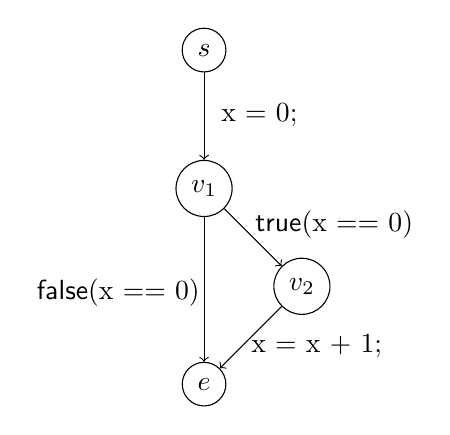
\begin{tikzpicture}[node distance={50pt}, main/.style = {draw, circle}] 
      \node[main] (0) {$s$};
      \node[main] (1) [below of=0] {$v_1$};
      \node[main] (2) [below right of=1] {$v_2$};
      \node[main] (3) [below left of=2] {$e$};
      \draw[->] (0) -- node[midway, xshift=20pt, yshift=16pt, pos=1] {x = 0;} (1);
      \draw[->] (1) -- node[midway, xshift=19pt, yshift=15pt, pos=1] {\textsf{true}(x == 0)} (2);
      \draw[->] (2) -- node[midway, xshift=35pt, yshift=8pt, pos=1] {x = x + 1;} (3);
      \draw[->] (1) -- node[midway, xshift=-31pt, yshift=25pt, pos=1] {\textsf{false}(x == 0)} (3);
    \end{tikzpicture}
  \end{subfigure}
  \caption{Example program (left) and corresponding CFG (right)}
  \label{fig:example_cfg}
\end{figure}

  \section{Related Work}
  % TODO: Related Work
  \section{Static Analysis}
  Static analysis is defined by Rival~\cite{rival2020introduction} as "[...]an automatic technique that approximates in a conservative manner semantic properties of programs before their execution". This means that the program is analyzed just by the given source code without execution. The goal is to prove certain properties about the program in a "sound" manner i.e. any property that is proven to hold actually does hold. However, from failing to prove a property one cannot conclude that the given property does not hold.\\
  In order to prove properties, e.g. finding that a program does not contain races or identifying dead code, we need to gain information about the program. This is done by performing various kinds of analyses. We will focus on flow sensitive analyses from now on i.e. analyses which find properties of the program dependent on the location within it. The semantic of these will be introduced in the following chapters.
  
    \subsection{Flow sensitive analysis}

    As noted above flow sensitive analyses find properties of the program dependent on the point within the program. Expressed differently this means a flow sensitive analysis will find an overapproximation of states the program may be in for any given point within the program or "program point". This state can describe many things dependent on the analysis performed.\\
    First let us define what a program point is: Imagine a control flow graph (CFG), where nodes represent points between instructions within the program. Edges are labeled with instructions or checks and describe the transitions between these points (see example \ref{fig:example_cfg}). Then any node on this CFG would be what we call a program point.\\
    Concretely let $N$ be the set of all program points. Furthermore, let $\mathbb{D}$ be a Domain containing abstract states describing concrete states of the program. This means that some $d \in \mathbb{D}$ can describe many states the program can be in.\\ 
    Then an analysis is expected to find a mapping $\eta: N \rightarrow \mathbb{D}$ which maps program points to abstract states describing that location within the program i.e. for $[n] \in N$, $\eta\ [n]$ should be an abstract state describing all possible states (and possibly more) the program can be in at program point $[n]$.\\
    As an example we will introduce a values-of-variables analysis for integers. This analysis finds a mapping from a set of variables $X$ to abstractions of their possible values at any given program point. In the scope of this thesis we will focus on abstracting integer values by sets of integers. Thereby the goal of our values-of-variables analysis is to find a mapping $X \rightarrow 2^\mathbb{N}$ for each program point.\\
    Combining this with the semantic of flow sensitive analysis from before, we get that the Domain $\mathbb{D}_v$ for the values-of-variables analysis should be $\mathbb{D}_v = X \rightarrow 2^\mathbb{N}$. Finally, the resulting $\eta_v: N \rightarrow \mathbb{D}_v$ for this analysis describes a mapping $\eta_v\ [n]$ for some program point $[n] \in N$, where $\eta_v\ [n]\ x$ is a set containing all values $x \in X$ may possibly hold at $[n]$. From this we can conclude that $x$ cannot hold any value outside $\eta_v\ [n]\ x$ at program point $[n]$.

    \subsection{Constraint systems}
    We now formulate a way in which we can describe an analysis in the form of constraints. For this we need a partial ordering $\sqsupseteq$ on the domain $\mathbb{D}$.\\
    Then we create a system of constraints which can be solved for a solution. Consider the edges $(u, A, v)$ of the CFG, where each edge denotes a transition from program point $[u]$ to program point $[v]$ via the instruction $A$. Now let each of these edges give raise to a constraint $\eta\ [v] \sqsupseteq [\![A]\!]^{\#}\ (\eta\ [u])$, where $[\![A]\!]^{\#}$ denotes the abstract effect of the instruction or check $A$ defining our analysis. In addition we need a start starte. this is usually the maximal element according to our ordering, giving raise to the start constraint $\eta\ [s] \sqsupseteq \textsf{max}(\sqsupseteq,\mathbb{D})$.

  



